% Čo by mala kapitola obsahovať
% - popísať ako sa pracuje s jednotlivými aplikáciami z pohľadu používateľa, aj screenshoty
% - popísať kritériá, tabuľka s kritériami - use casy
% - popísať slovne ako jednotlivé aplikácie spĺňajú dané kritériá 
% - tabuľka s porovnaním aplikácií vrátane mojej 
\chapter{Existing solutions}
Now that we have stated what shall the application do, we will discuss the currently available solutions which solve similar problems to our application.
In this chapter we are going to show applications and how a user can use them.
After that, we will describe criteria with which we will describe these applications and measure how the applications achieve these criteria.
Then ... a table where are all application are compared with our application.

\section{Overview of existing similar applications}
We are going to look at available existing applications which are similar to our application.

\subsection{Allergy Menu}
Allergy Menu provides restaurant guests with interactive menus.
There are allergen icons in the menu item's description.
A guest can interact with the menu by choosing what allergens they want to avoid.
A guest can also select an option that they are either a vegan or vegetarian.
The application filters out items of a menu to meet the guest's preferences.
The application allows a restaurant employee create a menu and specify what allergens are contained in each item of the menu.

\begin{figure}[h]
  \centering
  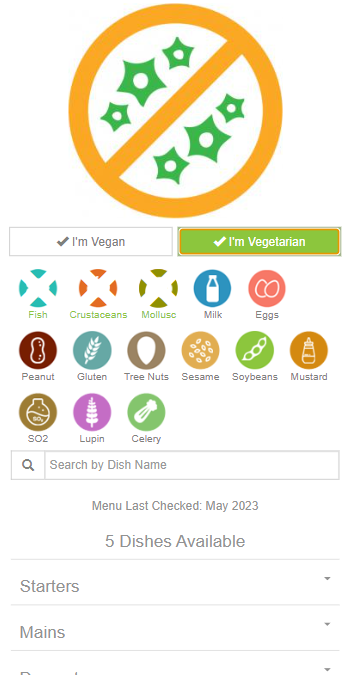
\includegraphics[width=0.62\linewidth]{master-thesis/img/allergen_menu_screenshot.png}
  \caption{The Allergy Menu application}
\end{figure}

\section{Comparison of the applications}

% \section{Other applications worth mentioning}
